% !TeX root = ../thesis.tex

\section{Architecture}
The architecture of the \velocity{} framework consists of seven steps that are performed sequentially in a pipeline fashion, as illustrated in the sequence diagram (\autoref{fig:velocity-sequence-diagram}). Every step is executed by one of three individual components, which will now be introduced briefly.

\begin{figure}[htbp!]
	\centering
	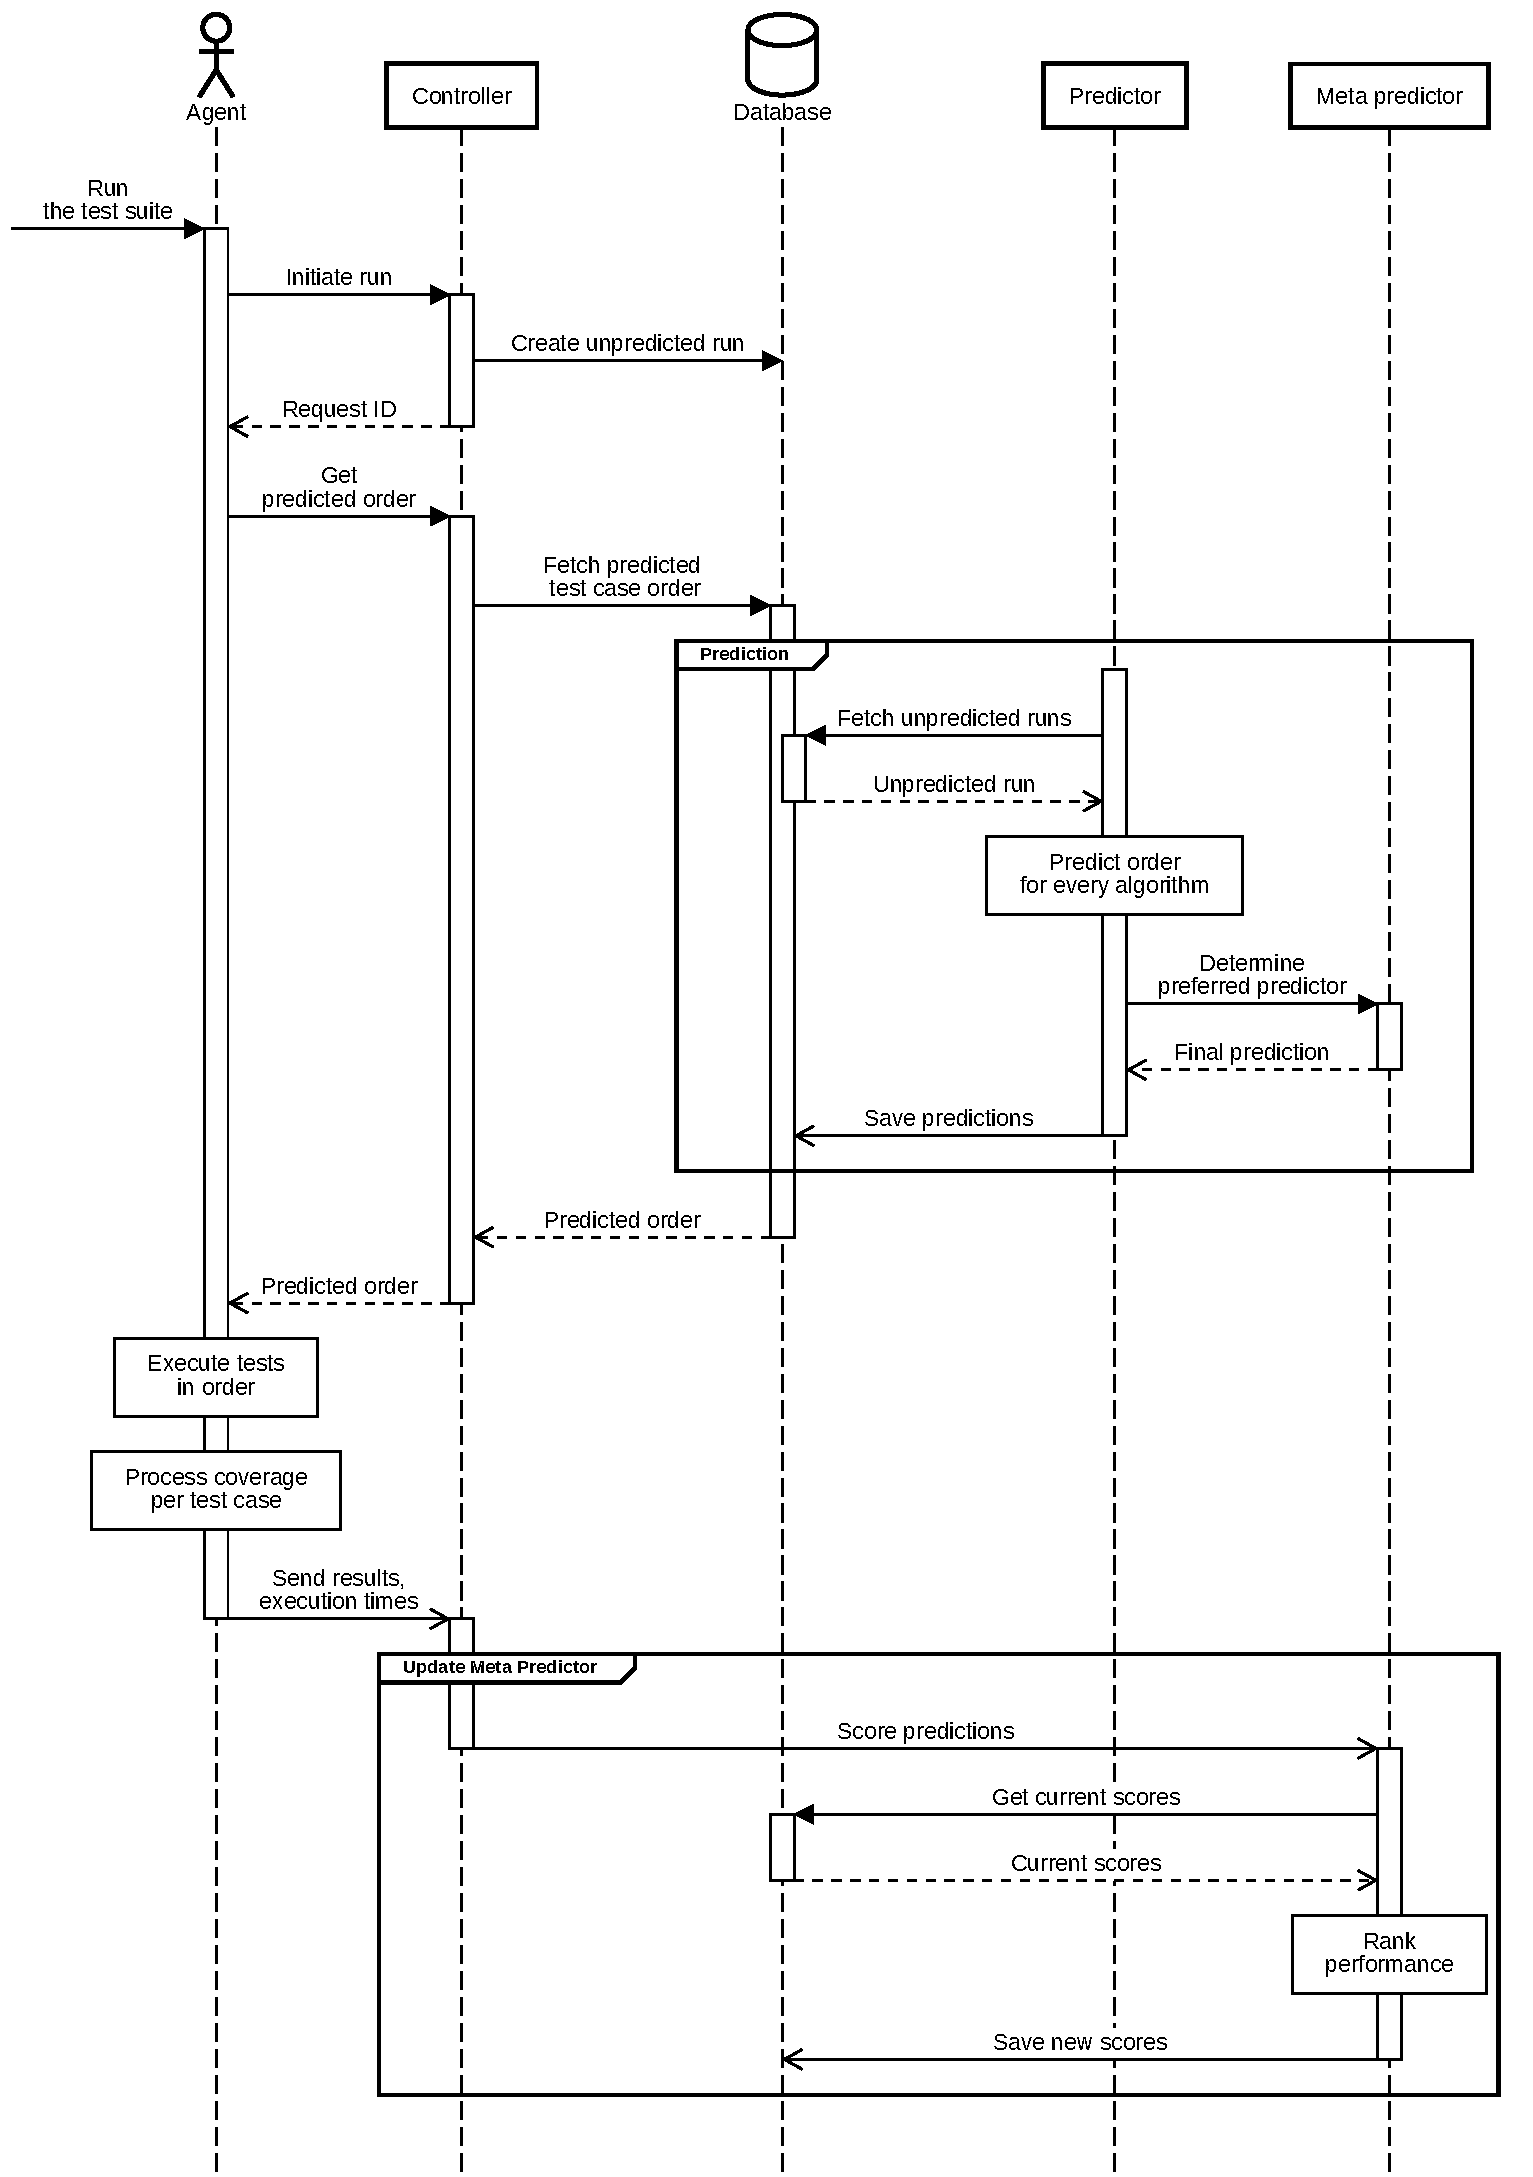
\includegraphics[width=\textwidth]{assets/diagrams/sequence-diagram.pdf}
	\caption{Sequence diagram of \velocity{}}
	\label{fig:velocity-sequence-diagram}
\end{figure}

\subsection{Agent}
\label{ssec:velocity-frontend}
The first component that will be discussed is the agent. This is the only component that depends actively on both the programming language, as well as the used test framework, since it must interact directly with the source code and test suite. For every programming language or test framework that needs to be supported, a different implementation of an agent must be provided. This implementations are however strongly related, so much code can be reused or even shared. In this thesis, an agent was implemented in Java, more specifically as a plugin for the widely used Gradle and JUnit test framework. This combination was previously described in \autoref{ssec:relatedwork-gradle-junit}. This plugin is responsible for running the test suite in a certain prioritised order, which is obtained by communicating with the controller (\autoref{ssec:velocity-controller}). After the test cases have been executed, the plugin sends a feedback report to the controller, where it is analysed.

\subsection{Controller}\label{ssec:velocity-controller}
The second component is the core of the framework, acting as an intermediary between the agent on the left side and the predictor (\autoref{ssec:velocity-predictor}) on the right side. In order to satisfy the second design goal and allow language agnosticism, the agent communicates with the controller using the \texttt{HTTP} protocol by exposing a \emph{REST}-interface. Representational State Transfer \texttt{[REST]} is a software architecture used by modern web applications that allows standardised communication using existing HTTP methods. On the right side, the controller does not communicate directly with the predictor, but rather stores prediction requests in a shared database which is periodically polled by the predictor. Besides routing prediction requests from the agent to the predictor, the controller  will also update the meta predictor by evaluating the accuracy of earlier predictions of this project.

\subsection{Predictor and Metrics}\label{ssec:velocity-predictor}
The final component is twofold. Its main responsibility is to apply the prioritisation algorithms and predict an order in which the test cases should be executed. This order is calculated by first executing ten algorithms and subsequently picking the algorithm that has been preferred by the meta predictor. Additionally, this component is able to provide metrics about the test suite, such as identifying superfluous test cases by applying \tsm{}. More specifically, this redundancy is obtained using the greedy algorithm (\autoref{ssec:alg-greedy}). Both of these scripts have been implemented in Python, because of its simplicity and existing libraries for many common operations, such as numerical calculations (NumPy\footnote{\url{https://numpy.org/}}) and machine learning (TensorFlow\footnote{\url{https://www.tensorflow.org/}}).